\def\mytitle{Optimization Assignment}
\def\myauthor{Hari Venkateswarlu Annam}
\def\contact{hariannam99@gmail.com}
\def\mymodule{Future Wireless Communication (FWC)}
\documentclass[10pt, a4paper]{article}
\usepackage[a4paper,outer=1.5cm,inner=1.5cm,top=1.75cm,bottom=1.5cm]{geometry}
\twocolumn
\usepackage{graphicx}
\graphicspath{{./images/}}
\usepackage[colorlinks,linkcolor={black},citecolor={blue!80!black},urlcolor={blue!80!black}]{hyperref}
\usepackage[parfill]{parskip}
\usepackage{lmodern}
\usepackage{tikz}
\usepackage{physics}
\usepackage{tabularx}
\usetikzlibrary{calc}
\usepackage{amsmath}
\usepackage{amssymb}
\renewcommand*\familydefault{\sfdefault}
\usepackage{watermark}
\usepackage{lipsum}
\usepackage{xcolor}
\usepackage{listings}
\usepackage{float}
\usepackage{titlesec}
\providecommand{\mtx}[1]{\mathbf{#1}}
\titlespacing{\subsection}{1pt}{\parskip}{3pt}
\titlespacing{\subsubsection}{0pt}{\parskip}{-\parskip}
\titlespacing{\paragraph}{0pt}{\parskip}{\parskip}
\newcommand{\figuremacro}[5]{
    \begin{figure}[#1]
        \centering
        \includegraphics[width=#5\columnwidth]{#2}
        \caption[#3]{\textbf{#3}#4}
        \label{fig:#2}
    \end{figure}
}
\newcommand{\myvec}[1]{\ensuremath{\begin{pmatrix}#1\end{pmatrix}}}
\let\vec\mathbf
\lstset{
frame=single, 
breaklines=true,
columns=fullflexible
}
\thiswatermark{\centering \put(0,-105.0){
\includegraphics[scale=0.08]{iith_logo}} }
\title{\mytitle}
\author{\myauthor\hspace{1em}\\\contact\\IITH\hspace{0.5em}-\hspace{0.5em}\mymodule}
\date{}
\begin{document}
	\maketitle
\paragraph{\textit{Problem Statement}}- The line $y=mx+1$ is a tangent to the curvr $y^2=4x$ if the value of m is.

\section*{\large Solution}
\begin{figure}[H]
\centering
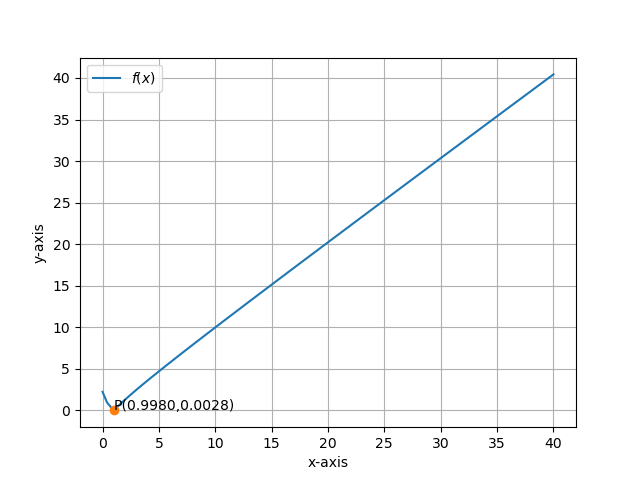
\includegraphics[width=1\columnwidth]{Figure1.png}
\caption{Graph of f(x)}
\label{fig:triangle}
\end{figure}

\begin{align}
\vec{x}^{\top}v\vec{x}+2\vec{u}^{\top}\vec{x}+f=0\\
\vec{n}^{\top}\vec{x}=1\\
\vec{x}=\vec{e_2}+\mu\vec{m}\\
d=\|\vec{n}\vec{x}-\vec{e_2}-{\mu}\vec{m}\|
\end{align}
    \subsection*{\normalsize Gradient descent}
    
    
    \begin{align}
	\label{eq:vol_varx}
	f(x) =\sqrt{\left(\frac{m^2x-2+m}{m^2}\right)^2+\left(\frac{2m\sqrt{x}-m-2+m}{m}\right)^2}
\end{align}
\begin{align}   
    f'(x) = \frac{(mx-\frac{2}{m}+1+2m-\frac{2}{\sqrt{x}})}{\sqrt{(mx-\frac{2}{m}+1)^2+(2m\sqrt{x}-2)^2}}
	\end{align}

we have to attain the maximum value of f(x). This can be seen in Figure f(x).Using gradient descent method we can find its minima value.
\begin{equation}
        x_{n+1} = x_n - \alpha \nabla f(x_n) \\
\end{equation}
\vspace{1mm}
\begin{equation}
\implies x_{n+1}=x_n+\alpha\frac{(mx-\frac{2}{m}+1+2m-\frac{2}{\sqrt{x}})}{\sqrt{(mx-\frac{2}{m}+1)^2+(2m\sqrt{x}-2)^2}}
\end{equation}

Taking $x_0=0.5,\alpha=0.001$ and precision = 0.00000001, values obtained using python are:
    

    \begin{align}
        \text{Minima} = 0.002824134040434986\\
        \implies \boxed{\text{Minima} = 0.002824134040434986}\\
        \boxed{\text{Minima Point} = 0.9980035344636117}
    \end{align}
    \begin{align*}
    \therefore  Hence\hspace{0.5em}Proved 
    \end{align*} 
   \end{document}
